%\documentclass{acmsiggraph}                     % final
\documentclass[annualconference]{acmsiggraph}  % final (annual conference)
%\documentclass[review]{acmsiggraph}            % review
%\documentclass[widereview]{acmsiggraph}        % wide-spaced review
%\documentclass[preprint]{acmsiggraph}          % preprint

%% Uncomment one of the five lines above depending on where your paper is
%% in the conference process. ``review'' and ``widereview'' are for review
%% submission, ``preprint'' is for pre-publication, and ``final'' is for
%% the version to be printed. The ``final'' variant will accept the 
%% ``annualconference'' parameter, which changes the height of the space
%% left clear for the ACM copyright information.

%% The 'helvet' and 'times' packages define the typefaces used for
%% serif and sans serif type in this document. Computer Modern Roman 
%% is used for mathematics typesetting. The scale factor is set to .92
%% to bring the sans-serif type in line with the serif type.

\usepackage[scaled=.92]{helvet}
\usepackage{times}

%% The 'graphicx' package allows for the inclusion of EPS figures.

\usepackage{graphicx}

%% use this for zero \parindent and non-zero \parskip, intelligently.

\usepackage{parskip}

%% Optional: the 'caption' package provides a nicer-looking replacement
%% for the standard caption environment. With 'labelfont=bf,'textfont=it',
%% caption labels are bold and caption text is italic.

\usepackage[labelfont=bf,textfont=it]{caption}
\usepackage{subfigure}

%% If you are submitting a paper to the annual conference, please replace 
%% the value ``0'' below with the numeric value of your OnlineID. 
%% If you are not submitting this paper to the annual conference, 
%% you may safely leave it at ``0'' -- it will not be included in the output.

\onlineid{0}

%% Paper title.

\title{A Work-Efficient GPU Algorithm for Level Set Segmentation}

\author{Mike Roberts\thanks{email: \{mlrobert,smcosta,rmitch\}@ucalgary.ca} \and Mario Costa Sousa^{*} \and Joseph Ross Mitchell^{*} }

\affiliation{University of Calgary}

\keywords{radiosity, global illumination, constant time}

%%%%%% START OF THE PAPER %%%%%%

\teaser{
  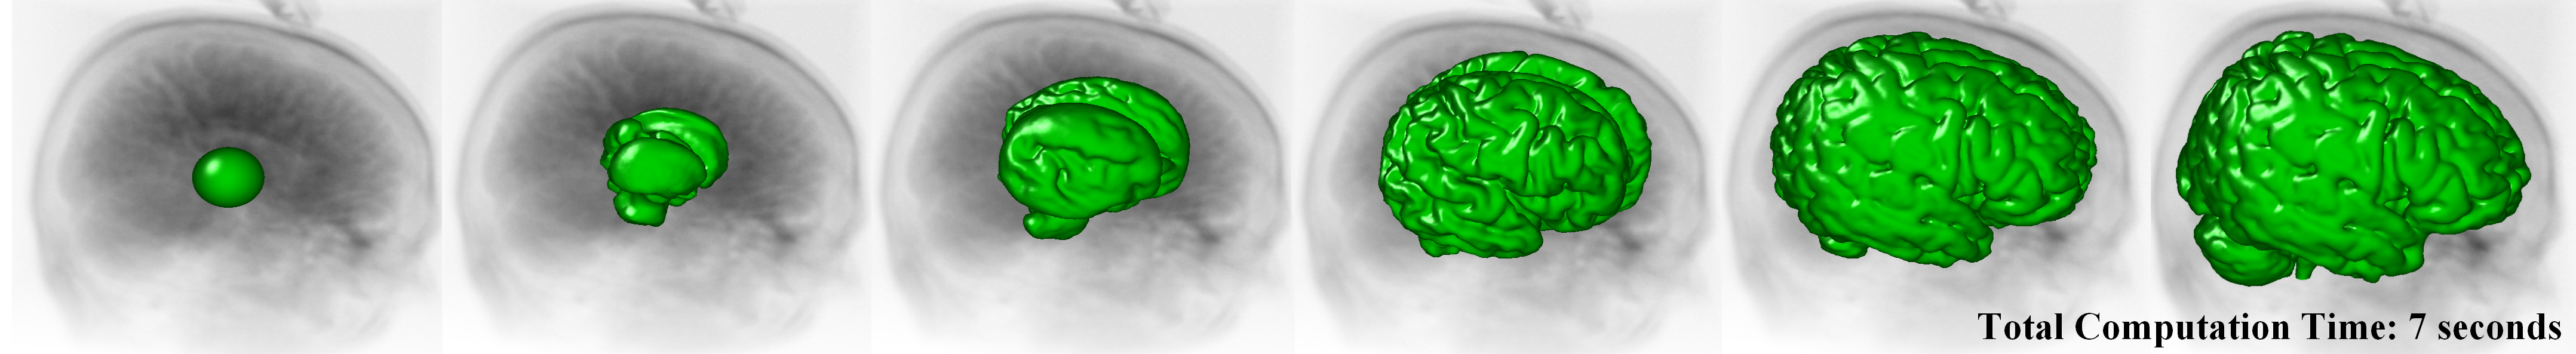
\includegraphics[width=7.0in]{figures/Brainweb-3D-Composite-1-6-text.png}
  \caption{The progression of our algorithm while segmenting the brain matter in a $256^3$ head MRI with a signal-to-noise ratio of 11. Our algorithm interactively computes this segmentation in 7 seconds -- 14$\times$ faster than previous GPU algorithms with no reduction in accuracy.}
  \label{fig:progression}
}
\begin{document}

\maketitle
\noindent{\textsf{\textbf{Abstract}}
We present a novel GPU level set segmentation algorithm that is both work-efficient and step-efficient. Our algorithm has $O(\log{n})$ step-complexity, in contrast to previous GPU algorithms~\cite{Lefohn-2004,Jeong-2009} which have $O(n)$ step-complexity. Moreover our algorithm limits the active computational domain to the minimal set of changing elements by examining both the temporal and spatial derivatives of the level set field. We apply our algorithm to 3D medical images (Figure \ref{fig:progression}) and demonstrate that our algorithm reduces the total number of processed level set field elements by $16 \times$ and is $14 \times$ faster than previous GPU algorithms with no reduction in segmentation accuracy.

\noindent{\textsf{\textbf{Introduction}}}
Identifying distinct regions in images -- a task known as \emph{segmentation} -- is an important task in computer vision and medical imaging. The GPU narrow band algorithm for level set segmentation can compute highly accurate segmentation results for noisy medical images and dramatically reduces computation times compared to optimized CPU implementations. However the GPU narrow band solver we tested took over 100 seconds converge on the brain matter in a ${256}^3$ head MRI on an Nvidia GTX 280 (Figure \ref{fig:performance}). This limitation constrains clinical applications and motivates our work-efficient algorithm.

The GPU narrow band algorithm avoids unnecessary computation by only updating field elements near the level set surface. We make the observation that even computations near the level set surface can be avoided in regions where the level set field has locally converged. This observation motivates our novel method of tracking the active computational domain.

\noindent{\textsf{\textbf{Our Algorithm}}}
We define the level set field value of an element $\mathbf{x}$ as $\phi(\mathbf{x})$. For each iteration, we initialize the active computational domain for the following iteration to be empty. Then for each currently active element $\mathbf{a}$, we check to see if $\nabla \phi(\mathbf{a})\neq 0$ and if there are any neighboring elements $\mathbf{n}$ around $\mathbf{a}$ (including $\mathbf{a}$ itself) such that $\frac{\delta \phi(\mathbf{n})}{\delta t} \neq 0$ where $t$ is simulation time. We add all such elements to the active computational domain for the following iteration.

We summarize our GPU algorithm for generating a new dense list of active elements from an old one as follows: (1) output new active elements in parallel such that each thread outputs all the new active elements in the neighborhood around one old active element; (2) remove all the duplicate active elements from step 1; (3) compact all the unique new active elements from step 2 into a new dense list.

In step 1 we output the neighbors along each cardinal direction into separate buffers. This guarantees that each buffer contains no duplicate elements. In step 2 we tag a 3D scratchpad buffer at all the left neighbors. For all the right neighbors we check if they're already tagged in the 3D scratchpad: if so we remove them remove them from the right neighbor buffer; if not we tag them in the 3D scratchpad. We repeat this process for all neighbor buffers. This process does not require sorting or any additional per-thread synchronization primitives (e.g atomic memory operations) since there are no duplicate elements in each neighbor buffer. In step 3 we use a work-efficient and step-efficient stream compaction algorithm \cite{Harris-2007} to compact each neighbor buffer.
\begin{figure}[t]
\centering
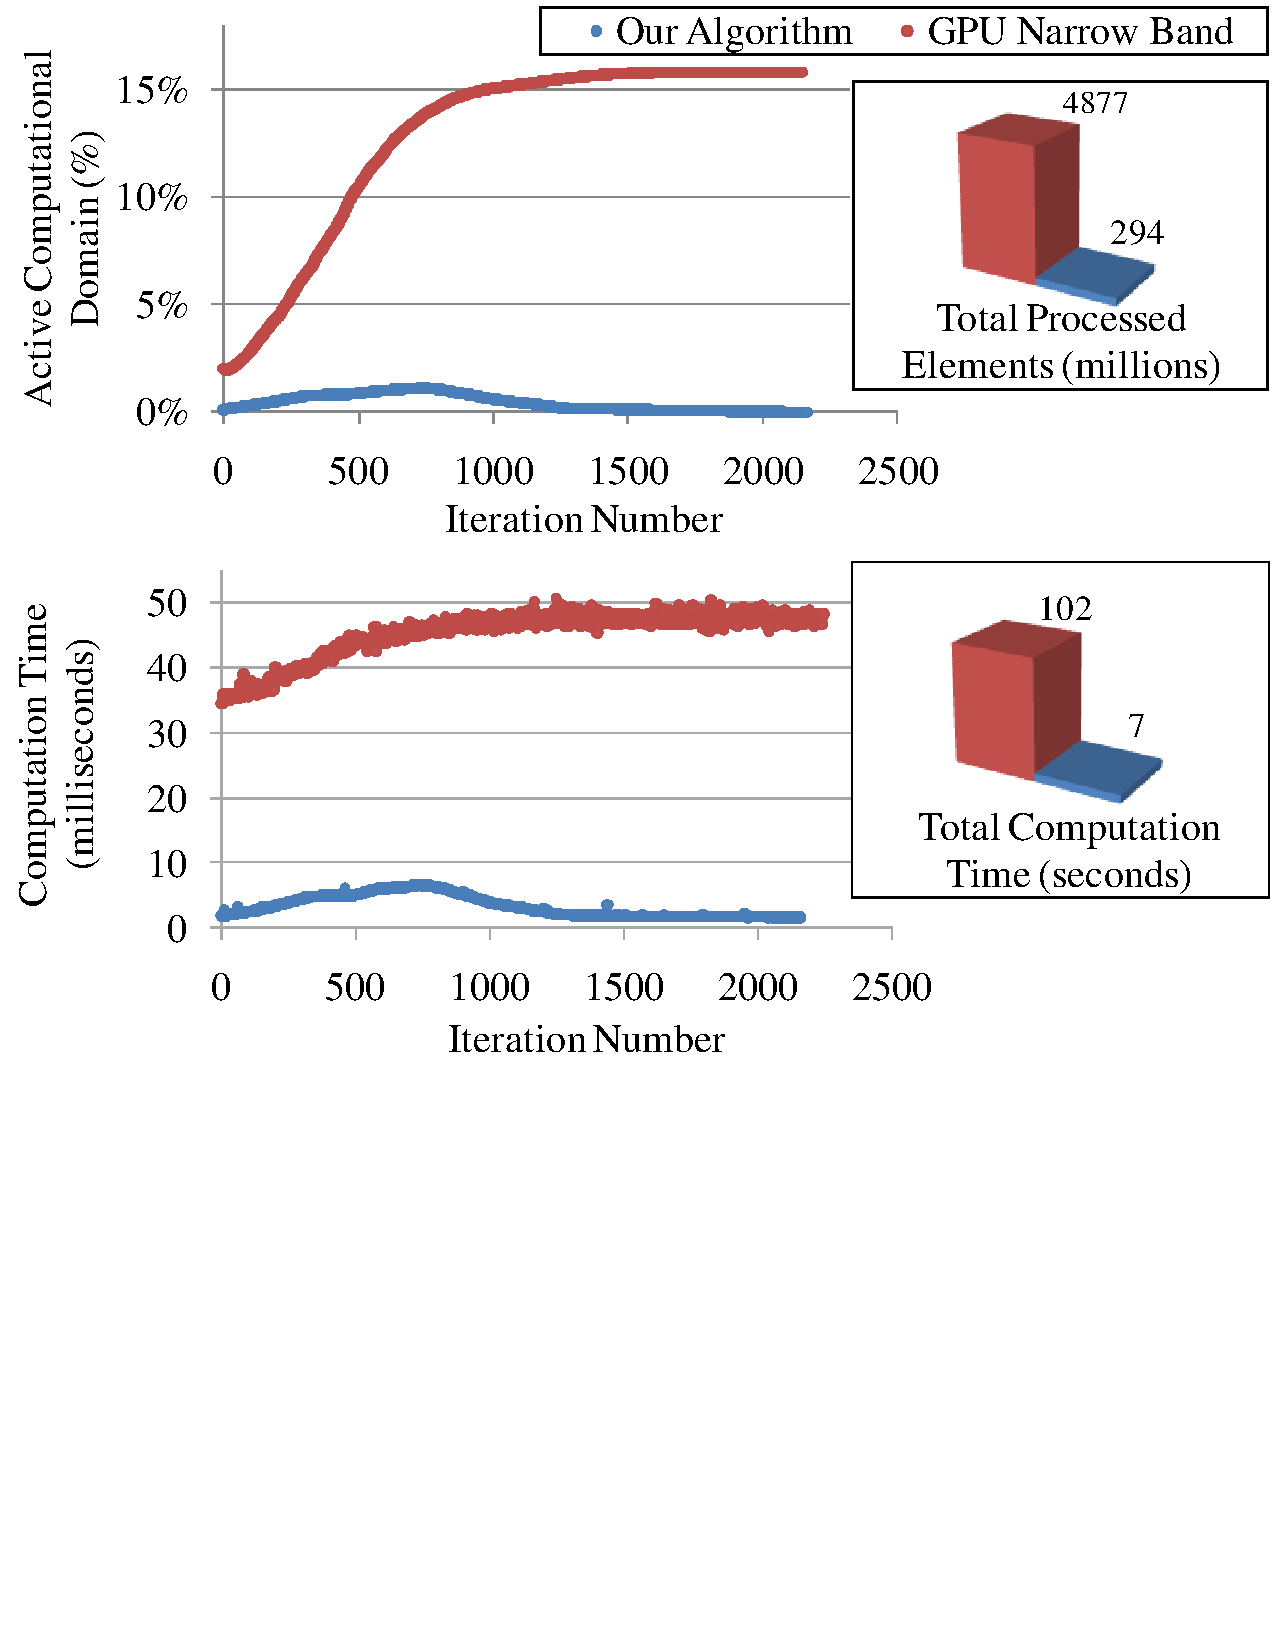
\includegraphics[width=3.3in]{figures/Performance-cropped.pdf}
\caption{ The active computational domain size (top) and speed (bottom) of our algorithm and the GPU narrow band algorithm while segmenting the brain matter in a $256^3$ head MRI. Both algorithms produced equally accurate segmentations. }
\label{fig:performance}
\end{figure}
\scriptsize{
\bibliographystyle{acmsiggraph}
\nocite{*}
\bibliography{template}
\end{document}
}
